\subsection{Evaluation}
   
   In order to estimate the cost of our algorithm, we want to model the time of an iteration at precision $b$. We model an iteration by the following formula: $an^3b^\alpha+c$, where $a,c$ and $\alpha$ are constants,
   $n$ is the size of the problem and $b$ the number of bits. Indeed, we expect the time to be proportional to the cube of the problem size as we deal with 3D problems, and the parameter $\alpha$ will characterize how the time evolves when we double the number of bits: if $\alpha = 1$, then multiplying by two the number of bits will multiply by two the cost of an iteration. Maybe the reality should be described by a more complicated polynomial in $b$, but we want to keep the model simple enough and see if the data can fit it.
   

%    To provide numerical values for $a$,$\alpha$ and $\beta$, we measured the execution times of different scenarios. Each scenario computes 50 iterations on a 64x64x64 matrix, on different processor topologies, and using
%    either only single-precision floating point variables or only double-precision floating point variables. We denote by $x_{b,n}$ the empirical value obtained using $b$ bits and $n$ processors. Results are reported in Table~\ref{table.time_measure1}.
%    \iffalse
%    P1x1x1, 10 iterations, average on ten runs\\
%    \begin{tabular}{|l|c|c|c|c|}
%    \hline
%     \multirow{2}{*}{Experiment} & \multicolumn{2}{c|}{Single-Precision} & \multicolumn{2}{c|}{Double-precision} \\
%     \cline{2-5}
%     & Solve (s) & Cycle (ms) & Solve (s) & Cycle (ms) \\
%     \hline
%     (1) 40x40x40 & 1.308 & 12 & 1.543 & 14\\
%     \hline
%     (1) 80x80x80 & 10.794 & 100 & 13.033 & 121.5\\
%     \hline
%     (2) 20x20x20 & 0.1316 & 1.1 & 0.1411 & 1.2 \\
%     \hline
%     (2) 40x40x40 & 1.026 & 9.5 & 1.195 & 11 \\
%     \hline
%     (2) 80x80x80 & 8.068 & 74 & 9.595 & 88 \\
%     \hline
%      (3) 20x20x20 & 0.170 & 1.4 & 0.179 & 1.5 \\
%     \hline
%      (3) 40x40x40 & 1.396 & 11.5 & 1.646 & 13.7 \\
%     \hline
%      (3) 80x80x80 & 10.644 & 89 & 12.572 & 106 \\
%     \hline
%      (4) 20x20x20 & 0.1405 & 1.2 & 0.149 & 1.3 \\
%     \hline
%      (4) 40x40x40 & 1.192 & 11 & 1.402 & 15\\
%     \hline
%      (4) 80x80x80 & 10.258 & 96 & 12.125 & 114 \\
%     \hline
%    \end{tabular}
%    
%    Jacobi\begin{tabular}{|l|c|c|c|c|}
%    \hline
%     \multirow{2}{*}{Experiment} & \multicolumn{2}{c|}{Single-Precision} & \multicolumn{2}{c|}{Double-precision} \\
%     \cline{2-5}
%     & Solve (s) & Cycle (ms) & Solve (s) & Cycle (ms) \\
%     \hline
%     (1) 40x40x40 & 0.0868 & 7.8 & 0.09577 & 8.4\\
%     \hline
%     (1) 80x80x80 & 0.709 & 63 & 0.8757 & 73\\
%     \hline
%     (2) 20x20x20 & 0.00945 & 0.8 & 0.00991 & 0.9 \\
%     \hline
%     (2) 40x40x40 & 0.0755 & 6.5 & 0.0815 & 7.2 \\
%     \hline
%     (2) 80x80x80 & 0.581 & 51 & 0.648 & 57 \\
%     \hline
%      (3) 20x20x20 & 0.0121 & 0.95 & 0.0126 & 1.0 \\
%     \hline
%      (3) 40x40x40 & 0.0990 & 7.8 & 0.105 & 8.2 \\
%     \hline
%      (3) 80x80x80 & 0.759 & 60 & 0.878 & 75 \\
%     \hline
%      (4) 20x20x20 & 0.0104 & 0.92 & 0.0106 & 1.0 \\
%     \hline
%      (4) 40x40x40 & 0.0842 & 7.6 & 0.0972 & 8.8\\
%     \hline
%      (4) 80x80x80 & 0.720 & 64.5 & 0.810 & 75.5 \\
%     \hline
%    \end{tabular}
% \fi
%   \begin{table}
%   \begin{center}
%    \begin{tabular}{|l|c|c|c|c|}
%    \hline
%     \multirow{2}{*}{Experiment} & \multicolumn{2}{c|}{Single-Precision} & \multicolumn{2}{c|}{Double-precision} \\
%     \cline{2-5}
%     & Solve (s) & Cycle (ms) & Solve (s) & Cycle (ms) \\
%     \hline
%     1x1x1 & 2.1853 & 70-80 & 2.6874 & 90 \\
%     \hline
%     2x1x1 & 1.3912 & 40-50 & 1.6476 & 50-60\\
%     \hline
%     2x2x1 & 0.8544 & 30-40 & 0.9943 & 40-50 \\
%     \hline
%     2x2x2 & 0.5393 & 10-20 & 0.6935 & 10-20 \\
%     \hline
%     4x2x2 & 0.3255 & 0-10 & 0.3802 & 10 \\
%     \hline
%     4x4x2 & 0.2542 & 0-10 & 0.2815 & 0-10 \\
%     \hline
%     4x4x4 & 0.3171 & 0-10 & 0.362 & 0-10 \\
%     \hline
%    \end{tabular}
%    \end{center}
%    \caption{Execution times of AMG solver using either single or double precision.}
%    \label{table.time_measure1}
%  \end{table}
%    
%    The first thing to notice is that increasing the number of processors decreases the execution times, except when going from 32 to 64. This is because the matrix becomes very small and the communication costs become too important.
%    We won't use theses two values for what follows.
%    We now need to find values of $a,\alpha$ and $\beta$ that fit our measures.\\
%    We will change from $a$ to a new $a'$ by setting $f(b,n) = \frac{a'}{n^\beta} \left(\frac{b}{32}\right)^\alpha$. Now if we look only at the 6 points for $b=32$, we just have $f(32,n) = \frac{a'}{n^\beta}$, which does not
%    depend on $\alpha$. To fit our data, we evaluate the least squares sum, that is to say $\sum\limits_{i=0}^5 (f(32,2^i)-x_{32,2^i})^2$. We want it to be minimized, so choosing the best $a$ is done by choosing
%    $\frac{x_{32,1}*1^\beta + \dots + x_{32,32}*32^\beta}{6}$. Then the minimal sum is obtained for $\beta \approx 0.634$, giving $a' \approx 2.099$.\\
%    Finally, we evaluate the least squares sum using all the 12 values to find the value of $\alpha$. The result found in this case is $\alpha \approx 0.3157$. To come back to the original formula we just have to divide $a'$ by $32^\alpha$, and we obtain
%    the final following formula:
%    \[ f(b,n) \approx \frac{0.703}{n^{0.634}} b^{0.3157}. \]
%    
%    Now that we modeled how time increases when $b$ incrases, we can evaluate different strategies that use.
%    
%    \iffalse
%    (1) 64x64x64, 50 iterations, averaged on 100 runs (Jacobi)\\
%    \begin{tabular}{|l|c|c|c|c|}
%    \hline
%     \multirow{2}{*}{Experiment} & \multicolumn{2}{c|}{Single-Precision} & \multicolumn{2}{c|}{Double-precision} \\
%     \cline{2-5}
%     & Solve (s) & Cycle (ms) & Solve (s) & Cycle (ms) \\
%     \hline
%     1x1x1 & 1.3731 & 40-50 & 1.6986 & 50-60\\
%     \hline
%     2x1x1 & 0.9028 & 30 & 1.1481 & 40-60\\
%     \hline
%     2x2x1 & 0.593 & 20 & 0.7015 & 30-40 \\
%     \hline
%     2x2x2 & 0.3762 & 10 & 0.5316 & 10-20 \\
%     \hline
%     4x2x2 & 0.2447 & 0-10 & 0.2681 & 0-10 \\
%     \hline
%     4x4x2 & 0.2032 & 0-10 & 0.2362 & 0-10 \\
%     \hline
%     4x4x4 & 0.3086 & 0-10 & 0.3477 & 0-10 \\
%     \hline
%    \end{tabular}
%   \fi
%   
%     \includegraphics[width=\textwidth]{figs/3157_3.pdf}\\
%     \includegraphics[width=\textwidth]{figs/3157_5.pdf}\\
%     \includegraphics[width=\textwidth]{figs/3157_7.pdf}\\
%     \includegraphics[width=\textwidth]{figs/3157_10.pdf}\\
%     \includegraphics[width=\textwidth]{figs/3157_15.pdf}

   To provide numerical values for $a,c$ and most importantly $\alpha$, we measure the execution times of different scenarios. Each scenario computes 50 iterations on matrices with different sizes, and using
   either only single-precision floating point variables or only double-precision floating point variables. We denote by $x_{b,n}$ the empirical value obtained using $b$ bits and a problem of size $n$ (i.e. the matrix
   considered will be of size $n^3 \times n^3$ as we consider 3D problems). %Results are reported in Table~\ref{table.time_measure1}.
   
   Then, using Python's lmfit package, we interpolate the data to find good values for $a,c$ and $\alpha$. We are able to estimate different values of $\alpha$, all between 0.20 and 0.32, using 3
   different applications, 2 types of cycles (the classic V-cycle and the \emph{Up} strategy) and 2 types of relaxation method (weighted Jacobi and an hybrid method). Each data-fitting was done on either 30 or 40 points.
   With these values of $\alpha$, we can estimate the cost of our algorithm in units of time by $\left(\frac{b}{53}\right)^\alpha$ for a cycle (1 unit = 1 V-cycle at double-precision) with $b$ the number of significant
   bits (i.e. the number of bits in the mantissa plus one, as one bit is always assumed in standard floating point representation). Then using the MPFR library we can create different
   scenarios that set the number of bits used at each cycle in a different way. We define all these scenarios by the first precision ($b$ in the manstissa)) used and how to update it ($delta$ bits added in the mantissa when the threshold is reached for a given precision).
   Strategies are denoted as $b\_delta$.
   This can be either an addition or a multiplication. In particular, we provide a scenario where the available precisions are 11, 24 and 53 (represented by a starting precision of 11 and a multiplicator of 2.24). This
   corresponds to the case where half-precision, single-precision and double-precision floating points are available, as it is the case on GPUs.
   
   \begin{figure*}
    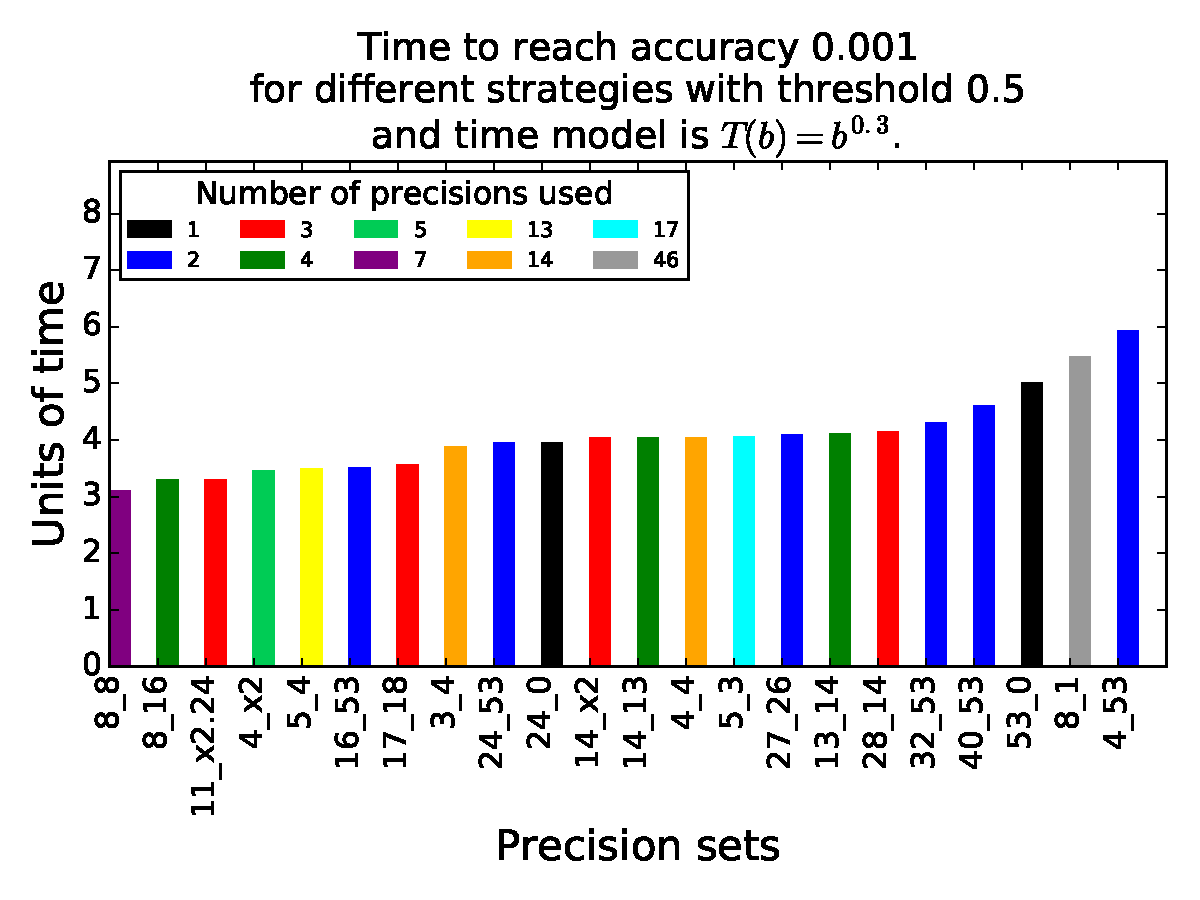
\includegraphics[width=0.33\linewidth]{figs/cost_3.pdf}
    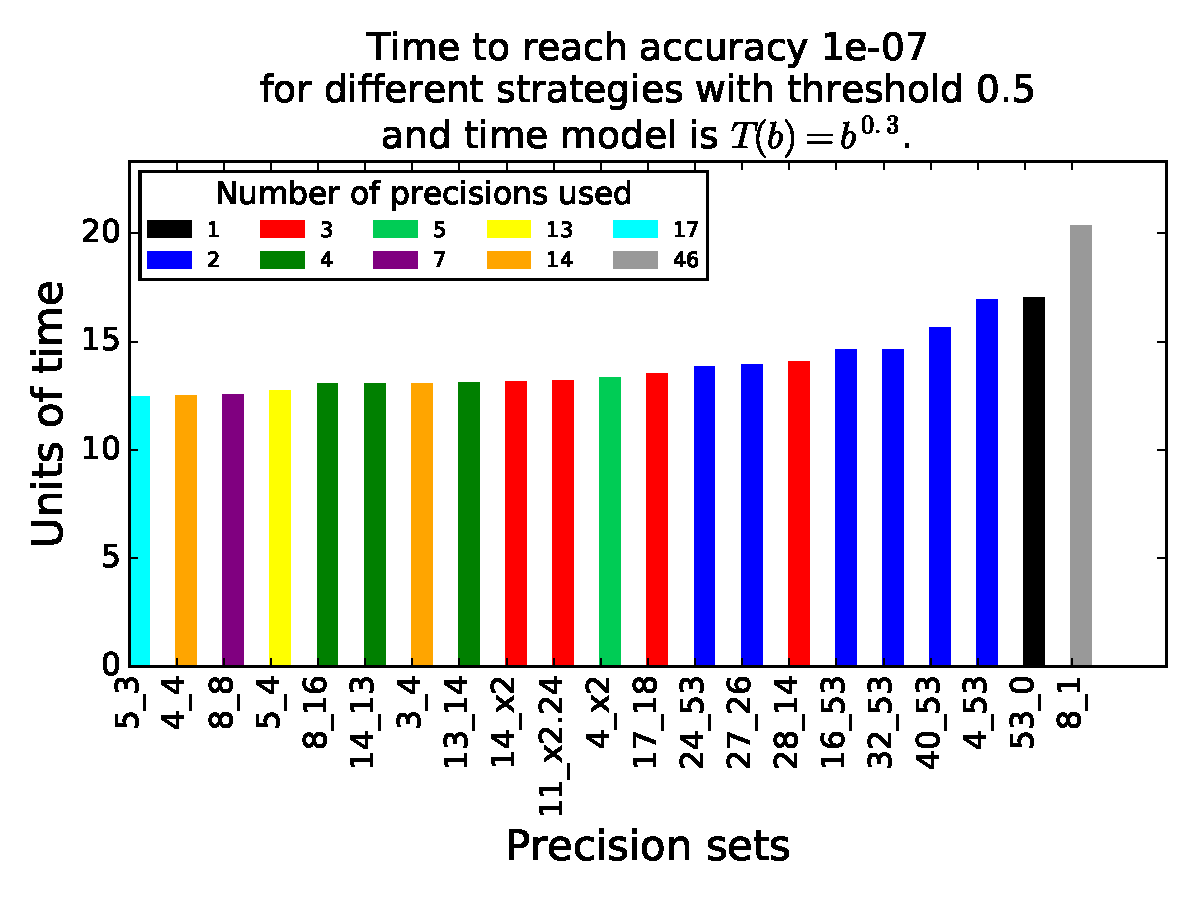
\includegraphics[width=0.33\linewidth]{figs/cost_7.pdf}
    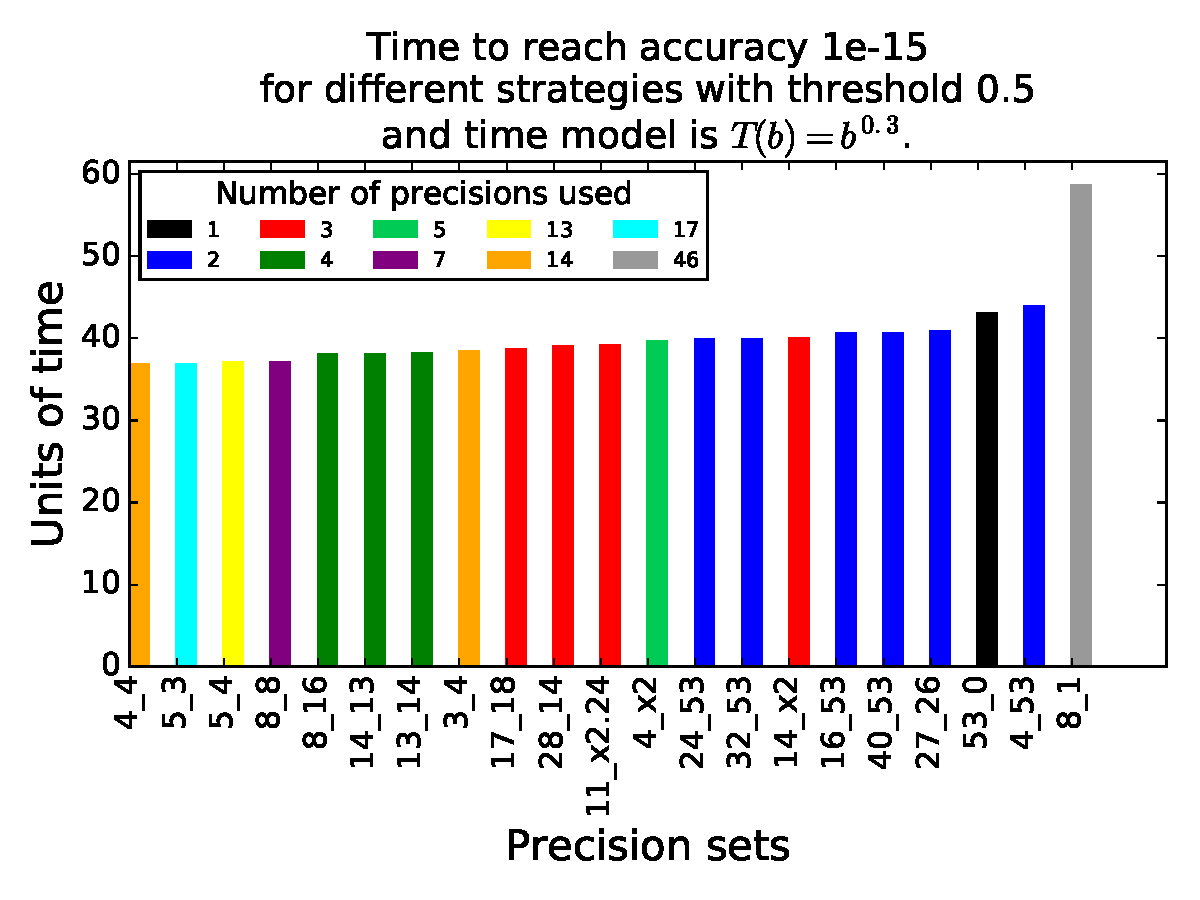
\includegraphics[width=0.33\linewidth]{figs/cost_15.pdf}
    \caption{Cost of the MG solver considering several different dynamic accuracy scenarios to reach different error degrees in the output: $10^{-3}$ on the left, $10^{-7}$ in the middle and $10^{-15}$ on the right.}
    \label{fig.estimation1}
   \end{figure*}
   %\begin{figure}
   % 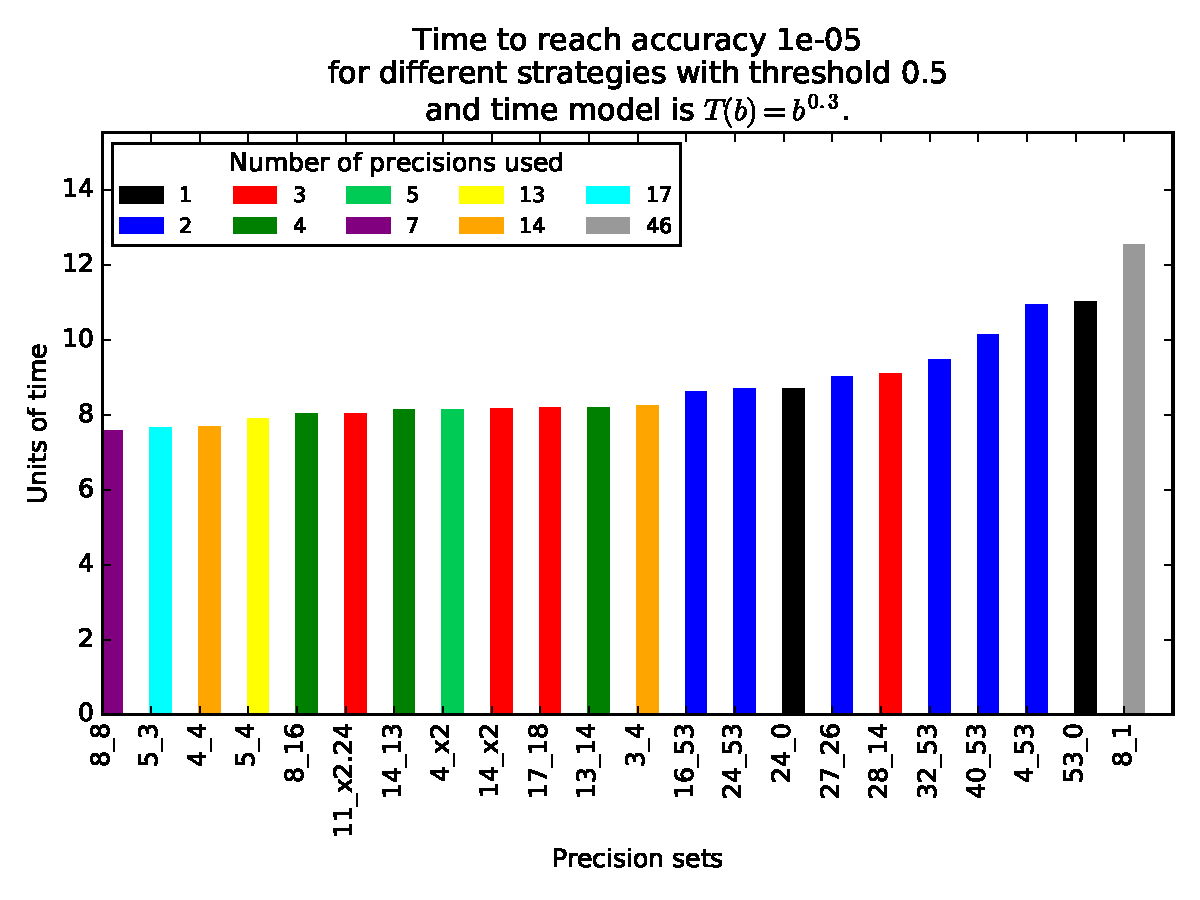
\includegraphics[width=\linewidth]{figs/cost_5.pdf}
   % \caption{}
   % \label{fig.estimation2}
   %\end{figure}
   %\begin{figure}
   % 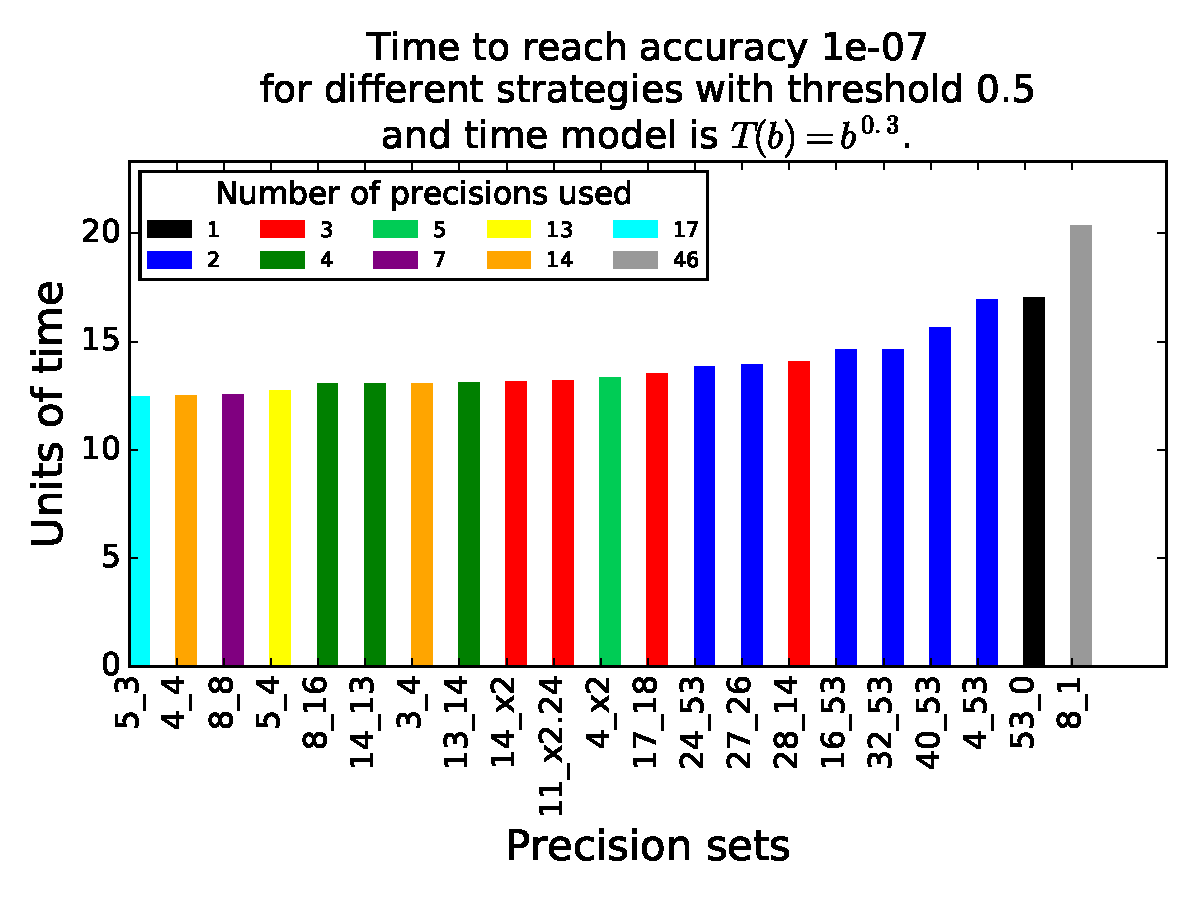
\includegraphics[width=\linewidth]{figs/cost_7.pdf}
   % \caption{}
   % \label{fig.estimation3}
   %\end{figure}
   %\begin{figure}
   % 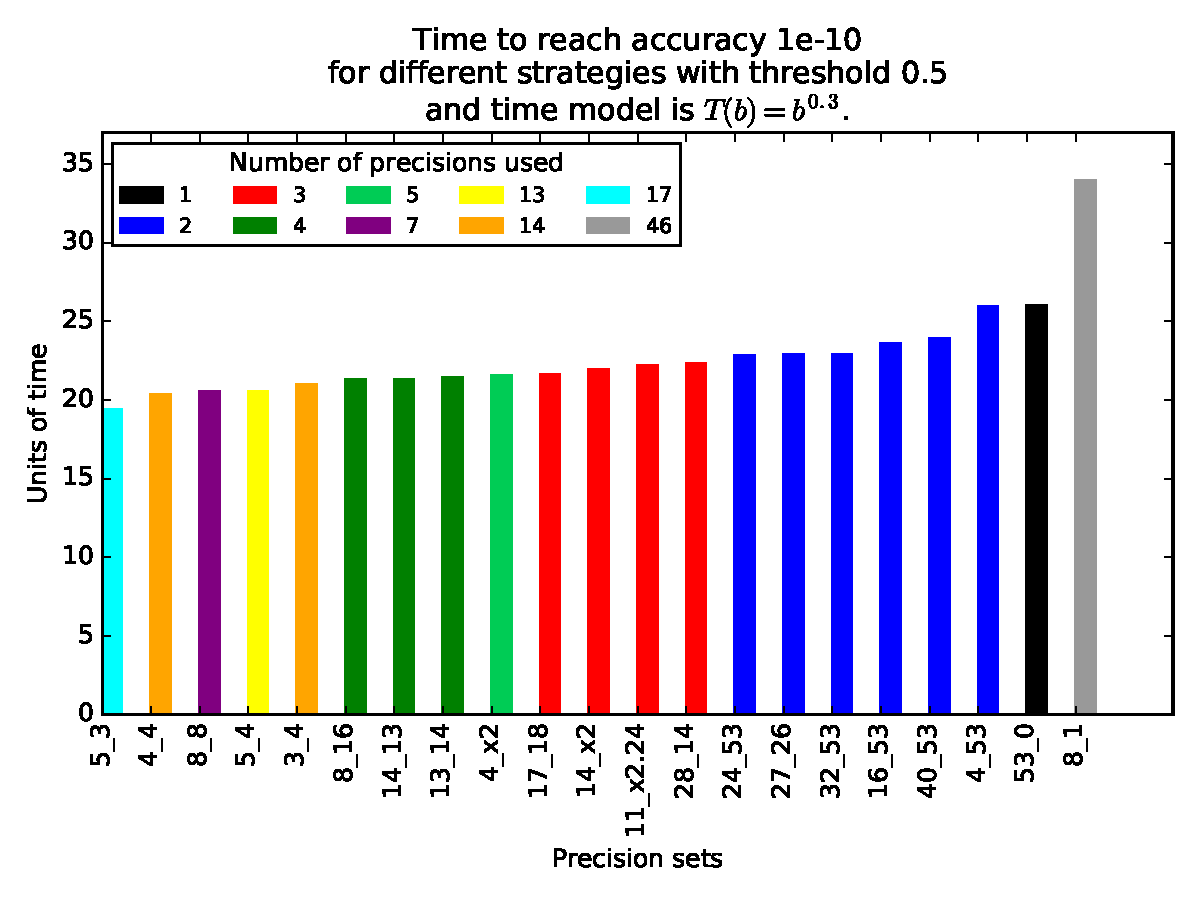
\includegraphics[width=\linewidth]{figs/cost_10.pdf}
   % \caption{}
   % \label{fig.estimation4}
   %\end{figure}
   %\begin{figure}
   % 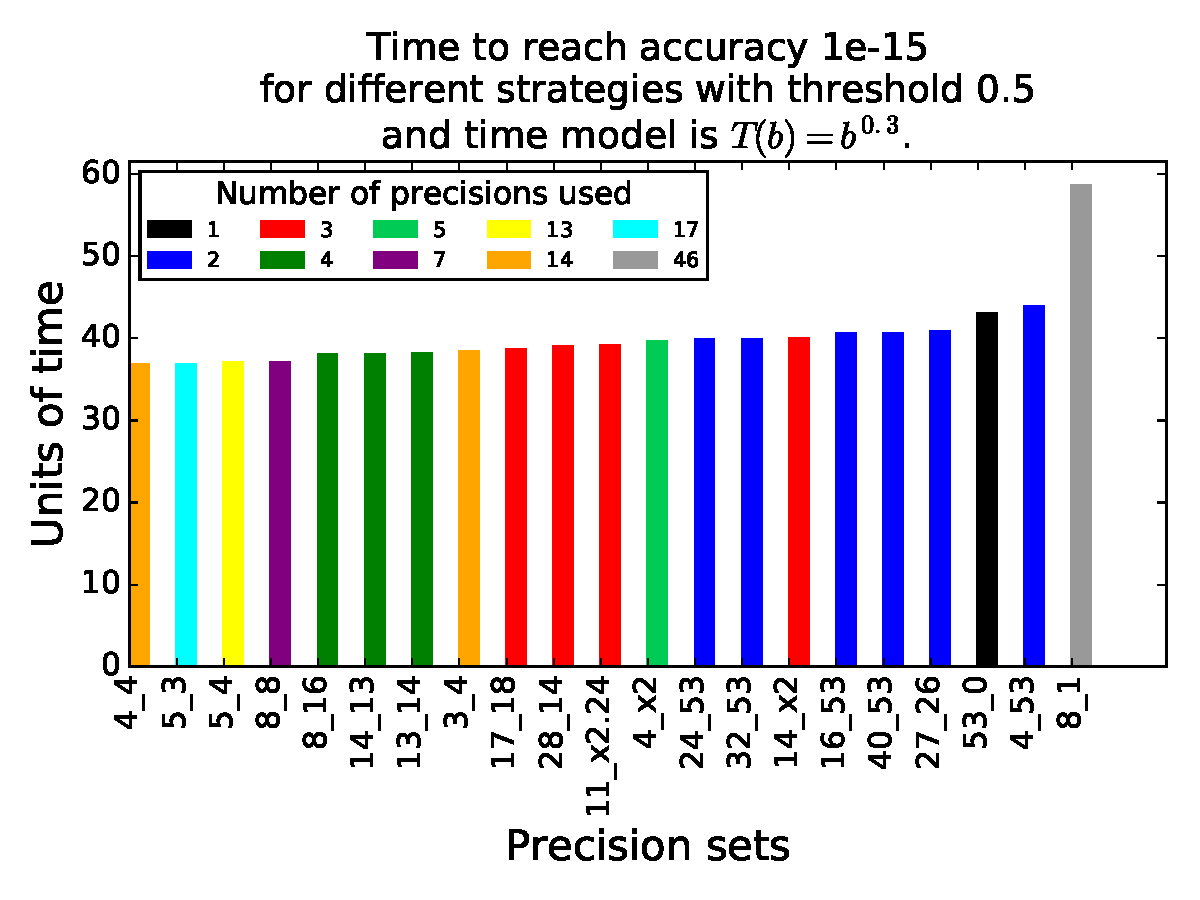
\includegraphics[width=\linewidth]{figs/cost_15.pdf}
   % \caption{}
   % \label{fig.estimation5}
   %\end{figure}
   
   Figure~\ref{fig.estimation1} represents the cost of the MG solver, for these different scenarios, to reach different accuracy degrees in the output ($10^{-3}$ on the left, $10^{-7}$ in the middle and $10^{-15}$ on the right) using
   a value for the $\alpha$ parameter of 0.3. We can see that the strategy that increases by only 1 the number of mantissa bits (labelled \texttt{8\_1}) takes more time than the original algorithm (labelled \texttt{53\_0}) for the 5 different accuracies presented. This is because, in the previous experiments we saw
   there is usually the same number of cycles in all our strategies (see Figure~\ref{fig.prec_incr}). Here, the convergence rate is limited by the slowly increasing number of precision bits: by adding one bit we can divide by at most 2 the 
   accuracy on the residual norm while the original algorithm can divide by more than that in one cycle if it is not limited by the bitwidth of the variables.
   If we focus on a case starting with half precision, then going to single and finally to double precision (labelled \texttt{11\_x2.24}), we can see that, compared to the original algorithm (which uses only double-precision), we improve by 35\% the time to reach 
   accuracy $10^{-3}$ (see Figure~\ref{fig.estimation1}). If one adapts the algorithm to use only single-precision variables (labelled \texttt{24\_0}) as it would be sufficient to reach this accuracy, we would still reduce the time by 17\% (still Figure~\ref{fig.estimation1}). Then the improvement slowly decreases when increasing the accuracy to reach 10\% (for $10^{-15}$ on Figure~\ref{fig.estimation1}).
   
   \subsection{Summary of results}
   
   Finally, we want to see how changing the precisions during the algorithm also improves the execution time when we use the \emph{Up} strategy, defined in section~\ref{sec.assymetric}, compared to using the original algorithm (single or double precision).
   The table~\ref{table.results1} presents the different estimated times (in time units where 1 time unit is a V-cycle at double precision)
   for all 4 different algorithms: V-cycle (double precision), \emph{Up}-cycle (double precision), V-cycle (adaptive precisions 11-24-53), \emph{Up}-cycle (adaptive precisions 11-24-53) for Problem 1, using a hybrid relaxation method.
   We also present the improvement of the best method (i.e. \emph{Up}-cycle with different precisions) compared to the original algorithm (in double-precision and in single-precision when possible).
  
  \begin{table*}[t]
   \begin{center}
  \resizebox{\textwidth}{!}{
  \begin{tabular}{|c|c|c|c|c|c|c|}
    \hline
    Tolerance & Baseline (DP) & \emph{Up}-cycle (DP) & Adaptive (V-cycle) & Adaptive (\emph{Up}-cycle) & Improvement (DP) & Improvement (SP) \\
    \hline
    \hline
    1e-01 & 1.000 & 1.333 & 0.624 & 0.832 & 16.8\% & -5.5\%\\
    \hline
    1e-02 & 3.000 & 2.000 & 1.872 & 1.664 & 44.5\% & 29.7\%\\
    \hline
    1e-03 & 5.000 & 4.667 & 3.284 & 3.131 & 37.4\% & 20.6\%\\
    \hline
    1e-04 & 8.000 & 7.333 & 5.650 & 5.234 & 34.6\% & 17.0\%\\
    \hline
    1e-05 & 11.000 & 10.0 & 8.015 & 7.336 & 33.3\% & 15.4\% \\
    \hline
    1e-06 & 14.000 & 12.667 & 10.380 & 9.439 & 32.6\% & 14.5\%\\
    \hline
    1e-07 & 17.000 & 15.333 & 13.169 & 11.964 & 29.6\% & -\\
    \hline
    1e-08 & 20.000 & 18.000 & 16.169 & 14.631 & 26.8\% & -\\
    \hline
    1e-09 & 23.000 & 20.667 & 19.169 & 17.298 & 24.8\% & -\\
    \hline
    1e-10 & 26.000 & 24.000 & 22.169 & 20.631 & 20.7\% & -\\
    \hline
    1e-11 & 29.000 & 26.667 & 25.169 & 23.298 & 19.7\%& -\\
    \hline
    1e-12 & 32.000 & 29.333 & 28.169 & 25.964 & 18.9\% & -\\
    \hline
    1e-13 & 35.000 & 32.000 & 31.169 & 28.631 & 18.2\% & -\\
    \hline
    1e-14 & 38.000 & 34.667 & 34.169 & 31.298 & 17.6\% & -\\
    \hline
    1e-15 & 43.000 & 39.333 & 39.169 & 35.964 & 16.4\% & -\\
    \hline
  \end{tabular}
  }
  \end{center}
   \caption{All estimated times for Problem 1, size 40, hybrid relaxation method, on a single processor, with $\alpha = 0.3$. The column `Improvement (DP)' corresponds to
   the improvement between our adaptive algorithm using a \emph{Up}-cycle (column 5) compared to the original V-cycle with fixed double-precision (column 2). The column `Improvement (SP)' corresponds
   to the improvement between our adaptive algorithm using a \emph{Up}-cycle (column 5) compared to the original V-cycle with fixed single-precision.}
   \label{table.results1}
   \end{table*}
   
   The main result is that even to reach the maximum precision, we improve the execution time by more than 15\%. When it comes to smaller precisions, this improvement can be as high as 30\% compared to
   a single-precision algorithm and it even goes up to 45\% compared to the original double-precision version. We insist to remember that these results for the adaptive algorithm use 3 different precisions (11,24,53)
   whereas if other architectures would be available it would be possible to improve even more the execution by using more different precisions. For example, as we see on Figure~\ref{fig.estimation1}, using precisions
   4,8,12,16,\dots,48,52,53 should lead to a faster execution for reaching $10^{-15}$.
